\documentclass{article}
\usepackage[english]{babel}
\usepackage[utf8]{inputenc}
\usepackage{fancyhdr}
\usepackage{amsmath,amssymb,amsfonts,amsthm}
\usepackage{indentfirst}
\usepackage{bm}
\usepackage[a4paper, total={6in, 10in}]{geometry}

% For using subfigures
\usepackage{graphicx}
\usepackage{caption}
\usepackage{subcaption}

% To put a figure where it is
\usepackage{float}

\usepackage{tensor}
\usepackage{biblatex}
\usepackage{titlesec}
\usepackage{bbm, dsfont} % For indicator functions
\usepackage{mathtools} % for \coloneqq
\usepackage[bottom]{footmisc} % prevents pictures going below footnote :|
% \usepackage{pifont} % for \ding{...}

\addbibresource{../../articles/articles.bib}

% \newcommand\defeq{\stackrel{\mathclap{\normalfont\mbox{def}}}{=}}

\newcommand{\expect}[2][]{
\ifthenelse{\equal{#1}{}}{
\mathbb{E}\left[#2\right]
}{
\underset{#1}{\mathbb{E}}\left[#2\right]
}}

\newcommand{\cov}[2][]{
\ifthenelse{\equal{#1}{}}{
\text{Cov}\left[#2\right]
}{
\underset{#1}{\text{Cov}}\left[#2\right]
}}


\newcommand{\var}[2][]{
\ifthenelse{\equal{#1}{}}{
\text{Var}[#2]
}{
\underset{#1}{\text{Var}}[#2]
}}

\newcommand{\loss}[2][]{
\ifthenelse{\equal{#1}{}}{
\mathcal{L}(#2)
}{
\mathcal{L}_{#1}(#2)
}}

\newcommand{\kl}[2]{
\text{D}_\text{KL}[#1 \parallel #2]
}

\newcommand{\R}{\mathbb{R}}
%\newcommand{\Prob}{\mathbb{P}}

\newcommand{\1}[1]{\mathds{1}\{#1\}}

% We need this for \begin{theorem}...\end{theorem} staff
\newtheorem*{theorem*}{Theorem}
\newtheorem{theorem}{Theorem}
\newtheorem*{proposition*}{Proposition}
\newtheorem{proposition}{Proposition}
\newtheorem*{corollary*}{Corollary}
\newtheorem{corollary}{Corollary}
\newtheorem*{lemma*}{Lemma}
\newtheorem{lemma}{Lemma}
\newtheorem*{question*}{Question}
\newtheorem{question}{Question}

\theoremstyle{definition}
\newtheorem{definition}{Definition}[section]


\title{Information Bottleneck in Deep Learning}
\author{Ivan Skorokhodov}

\begin{document}

%\maketitle

\section{Information Theory basics}
Here we will give all the required definitions and their properties.

\begin{definition}
\textbf{Entropy} H(X) of a discrete random variable $X$ with probability mass function $p(X)$ is the quantity
\[
H(X) = \expect[p(x)]{-\log p(x)}
\]
\end{definition}

\begin{definition}
\textbf{Differential entropy} of a random variable $X$ with probability density function $p(x)$ is the quantity
\[
H(X) = \expect[p(x)]{-\log p(x)}
\]
\end{definition}

Mutual information:
\[
\begin{split}
I(X;Y)
&= H(X) - H(X|Y) \\
&= H(Y) - H(Y|X) \\
&= \kl{p(x,y)}{p(x)p(y)} \\
&= \text{TC}(p(x,y)) \\
&= \expect[x]{\kl{p(y|x)}{p(y)}}
\end{split}
\]

Chain rule for MI:
\[
I(X ; Y, Z)=I(X ; Z) + I(X ; Y | Z)
\]

Conditional MI identities:
\[
\begin{split}
I(X ; Y|Z)
&= \expect[Z]{\kl{p(x,y|z)}{p(x|z)p(y|z)}} \\
&= H(X, Z) + H(Y, Z) - H(X, Y, Z) - H(Z) \\
&= H(X|Z) - H(X|Y, Z) \\
&= H(X|Z) + H(Y|Z) - H(X, Y|Z) \\
\end{split}
\]

Conditional entropy:
\[
H_{p}(y | z) :=\mathbb{E}_{y, z \sim p(y, z)}[-\log p(y | z)]
\]

Conditional cross-entropy:
\[
H_{p, q}(y | z) := \mathbb{E}_{y, z \sim p(y, z)}[-\log q(y | z)]
\]


\section{Information Bottleneck as such}
\subsection{Origins and formulation}
Information Bottleneck origins from rate-distortion theory, which is solving the following task: given a random variable $X$ and some \textit{distortion} function $d(x,\tilde{x})$ quantize $X$ into $\tilde{X}$ such that $\tilde{X}$ is compressed as much as possible, but not too corrupted.
Strictly speaking, we are trying to solve
\[
\min_{p(\tilde{x} | x)} I(\tilde{X}; X) \quad \text{s.t. } D(X, \tilde{X}) \leq D^*,
\]
where
\[
D(X, \tilde{X}) = \expect[p(x, \tilde{x})]{d(x, \tilde{x})}
\]
and $D^*$ is the maximum value of possible distortion that we permit.
MSE loss or Hamming distance are common choices for $d(x, \tilde{x})$.

%We solve this problem by introducing lossy coding $X \xrightarrow{f} Z \xrightarrow{g} \tilde{X}$, where $f$ and $g$ are encoder and decoder.

%Why do we need it?
%Imagine you want to send a bag of memes to your grandma.
%Your grandma lives in countryside, where internet connection is quite week.
%

%Note, that here we minimize $I(\tilde{X}; X)$ and not $H(\tilde{X})$ which can feel more natural, is equivalent for deterministic mappings and actually being done sometimes.
%The reason for this is that (in discrete case) we are maximizing $H(X|\tilde{X})$ by doing this, and this means that we try to cover more $X$ with a single $\tilde{X}$.
%This, in turn, makes $\tilde{X}$ be set in those regions where $X$ is uniform and capture equal amounts of $X$.
%While minimization of $H(\tilde{X})$ can provide a solution, where TODO.

We can find optimal quantization by solving the variational problem:
\[
\loss{p(\tilde{x} | \tilde{x})} = I(X; \tilde{X}) + \beta D(X, \tilde{X})
\]

The main problem with rate-distortion theory is that we need a distortion function $d(x, \tilde{x})$, which is difficult to specify for complex structured data, such as video or speech.
And here Information Bottleneck comes to the rescue: what if after reconstruction we are only interested in some variable $Y$?
Then we can reformulate our problem as
\[
\loss{p(\tilde{x} | \tilde{x})} = I(X; \tilde{X}) - \beta I(Y, \tilde{X})
\]

For discrete case it can be shown \cite{Information_Bottleneck}, that it's a special case of rate-distortion problem with $d(x, \tilde{x}) = \kl{p(y|x)}{p(y|\tilde{x})}$.

\subsection{A few words about sufficient statistics}
\begin{itemize}
    \item Two datasets which give us the same inference about sufficient statistic, would give the same inference about underlying parameter $\theta$.
    \item Any injective function of sufficient statistic is also a sufficient statistic.
    \item Factorization theorem says, that $p(x|y) = h_T(X) g_T(T(X), y)$, dependence in $g_T$ in $x$ is only through $T(x)$.
\end{itemize}

\subsection{Sufficiency and minimality of representations}
From now on we'll use symbol $Z$ for variable $\tilde{X}$, because it's more consistent with modern DL literature.

We have the following optimization problem:
\[
\loss{p(x;z)} = I(X;Z) - \beta I(Z; Y)
\]

There is an interesting statement which connects notion of \textit{sufficiency} and \textit{minimality} of $Z$ in the $\beta \to \infty$ setting.
Let denote by $F(X)$ all random mappings of $X$ (this means, that for $f \in F(X)$ we have Markov chain $Y \to X \to f(X)$).
Let $S_Y(X)$ be a set of all sufficient statistics of $X$ for $Y$.

\begin{proposition}
If $Z$ is a solution to
\[
\min_{Z} I(X; Z) \quad\text{s.t. } I(Z;Y) = \max_{Z'} I(Z'; Y)
\]
then $Z$ is a minimal sufficient statistics of $X$ for $Y$
\[
P(X|Z,Y) = P(X|Z)
\]
\end{proposition}

In other words, we are getting a minimal sufficient representation by optimizing Lagrangian in the limit $\beta \to \infty$.
The proof of this theorem is split into two lemmas \cite{IB_learning_and_generalization}.

\begin{lemma}
    $Z$ is a sufficient statistic of $X$ for $Y$ iff $I(Z;Y) = I(X;Y)$.
\end{lemma}

\begin{proof}
Imagine that $T \in S_Y(X)$.
For any $Z \in F(X)$ we have a Markov chain $Y \to X \to Z$, so by DPI we have $I(Y;Z) \leq I(Y;X)$.
But by sufficient statistic property we have $P(X|Z,Y) = P(X|Y)$, so we have a Markov chain $Y \to Z \to X$.
Again by DPI we have $I(Y;Z) \leq I(Y;X)$, so $I(Y;Z) = I(Y;X)$.

Now consider $Z = f(X)$ for some $f \in F(X)$ such that $I(Y;Z) = I(Y;X)$.
As $Y \to X \to Z$ is a Markov chain, then by definition of conditional MI we have:
\[
\begin{split}
I(Y:Z|X) &\triangleq \expect[X]{\kl{p(Y,Z|X)}{p(Y|X)p(Z|X)}} \\
&= \expect[X]{\kl{p(Z|X,Y)p(Y|X)}{p(Y|X)p(Z|X)}} \\
&= \expect[X]{\kl{p(Y|X)p(Z|X)}{p(Y|X)p(Z|X)}} = 0
\end{split}
\]

Now, by chain rule for MI we have:
\[
I(Y : X,Z) = I(Y : Z) + I(Y,X|Z) = I(Y : X) + I(Y,Z|X) \Longrightarrow I(Y,X|Z) = I(Y,Z|X) = 0
\]
Applying definition of conditional MI again we get $p(Y,X|Z) = p(Y|Z)p(X|Z)$.
And this means that $Z \in S_Y(X)$:
\[
p(X|Y,Z) = \frac{p(X,Y|Z)}{p(Y|Z)} = \frac{p(X|Z) p(Y|Z)}{p(Y|Z)} = p(X|Z)
\]
\end{proof}

Let's denote by $S_Y^*(X)$ a set of minimal sufficient statistics of $X$ for $Y$.
\begin{lemma}
Let $Z \in S_Y(X)$, then
\[
Z \in S_Y^*(X) \Longleftrightarrow I(X;Z) = \min_{T \in S_Y(X)} I(X;T)
\]
\end{lemma}

\begin{proof}
First, let $Z$ be a minimal sufficient statistic.
Then for any other sufficient statistic $T$ we have $Z = f(T)$ for some $f$.
Then we get a Markov chain $X \to T \to Z$ and by DPI we have $I(X;Z) \leq I(X;T)$.

Now, let's prove reverse direction of the claim.
Imagine, that $Z \in S_Y(X)$ but is not minimal.
We are going to show, that $\exists T \in S_Y(X)$ such that $I(X;Z) > I(X;T)$.
By Fisher-Neyman factorization theorem we have
\[
Z \in S_Y(X) \Longleftrightarrow \exists\ h_Z, g_Z \text{ s.t. } \forall x,y \quad p(x|y) = h_Z(x) g_Z(Z(x), y)
\]

Let's define an equivalence relation
\[
a \sim b \Longleftrightarrow \forall y \exists \lambda s.t. \frac{g_Z(a, y)}{g_Z(b, y)} = \lambda(a, b)
\]

Now we define a deterministic function $T:\mathcal{X} \to \mathcal{Z}$ such that $\forall x: T(x) = \bar{z}$ --- a representative of $[Z(x)]$ (TODO: exists by axiom of choice?).
%This means that $T$ is a function of $Z$ and we have a Markov chain $X \to Z \to T$.
Let's prove, that it is a sufficient statistic.
For this let's define
\[
\begin{split}
h_T(x) &\triangleq h_Z(x) \frac{g_Z(Z(x), y)}{g_Z(T(x), y)} \\
g_T(T(x), y) &\triangleq g_Z(T(x), y)
\end{split}
\]
Then we have
\[
p(x|y) = h_Z(x) g_Z(Z(x), y) = h_Z(x) \frac{g_Z(Z(x), y)}{g_T(T(x), y)} g_T(T(x), y) = h_T(x) g_T(T(x), y)
\]
Hence $T$ is a sufficient statistic.

Now let's show that $I(X;Z) > I(X;T)$.
Since $Z$ is not minimal, then there is such $R \in S_Y(X)$ that $Z$ is not a function of $R$.
Let's show, that $T$ is a function of $R$ (btw, this will show, that $T$ is minimal).
For this we are going to show that if $R(x_1) = R(x_2)$ then $T(x_1) = T(x_2)$: this would allow us to build a function $\phi:\mathcal{R} \to \mathcal{T}$ which just take value $r$, find it's preimage $R^{-1}(r)$, take any sample $x \in R^{-1}(r)$ and compute $T(x)$.
For any $x_1, x_2$ such that $R(x_1) = R(x_2)$ we have:
\[
\begin{split}
\frac{g_Z(Z(x_1), y)}{g_Z(Z(x_2), y)}
&= \frac{p(x_1 | y) h_Z(x_2)}{p(x_2 | y) h_Z(x_1)} \\
&= \frac{h_R(x_1) g_R(R(x_1), y) h_Z(x_2)}{h_R(x_2) g_R(R(x_2), y) h_Z(x_1)} \\
&= \frac{h_R(x_1) g_R(R(x_1), y) h_Z(x_2)}{h_R(x_2) g_R(R(x_1), y) h_Z(x_1)} \\
&= \frac{h_R(x_1) h_Z(x_2)}{h_R(x_2) h_Z(x_1)} \\
&= \lambda(Z(x_1), Z(x_2))
\end{split}
\]
This means that $Z(x_1) \sim Z(x_2)$, which in turn means that $T(x_1) = T(x_2)$, so $T$ is minimal sufficient statistic and a function of $R$.
\end{proof}

\section{First steps: SZT experiments, critics}

\subsection{Main ideas}
First attempts to apply IB to deep learning are to Ravid Shwartz-Ziv and Naftali Tishby \cite{DL_and_IB}.
They proposed to view at a NN as a Markov chain
\[
Y \to X \to Z_1, ... , \to Z_l
\]
where $X$ is an input, and $Z_i$ is our hidden representations.

SZT theory claims that NNs implicitly minimizes IB Lagrangian for each layer and does the following claims:
\begin{itemize}
    \item There are two phases of training: fitting (when MI with input grows) and compression (when MI with input decreases).
    \item Compression results in good generalization.
    \item Compression occurs due to diffusion-like behaviour of SGD (looks like it was recently proved by \cite{SGD_and_VI_and_FP}).
\end{itemize}

They give nice pictures for this.
TODO: plot nice pictures of $I(X; Z_i)$ growing, then decreasing and $I(Z_i; Y)$ just growing.
Do not forget, that by DPI further layers should be lower for both $I(Z_i; Y)$ plot and $I(X;Y)$ plot as our Markov chain implies $y \to x \to z_1 \to ... \to z_l$.

We define SNR for SGD as
\[
\mathrm{SNR}=\frac{m_{l}}{s_{l}} \quad m_{l}=\left\|\operatorname{Mean}\left(\frac{\partial E}{\partial W_{l}}\right)\right\|_{F} \quad s_{l}=\left\|\operatorname{Std}\left(\frac{\partial E}{\partial W_{l}}\right)\right\|_{F}
\]

SZT claim that it this SGD behaviour was connected to fitting and compression phases.
Pictures on SNR for SGD looks like
\begin{figure}[H]
\centering
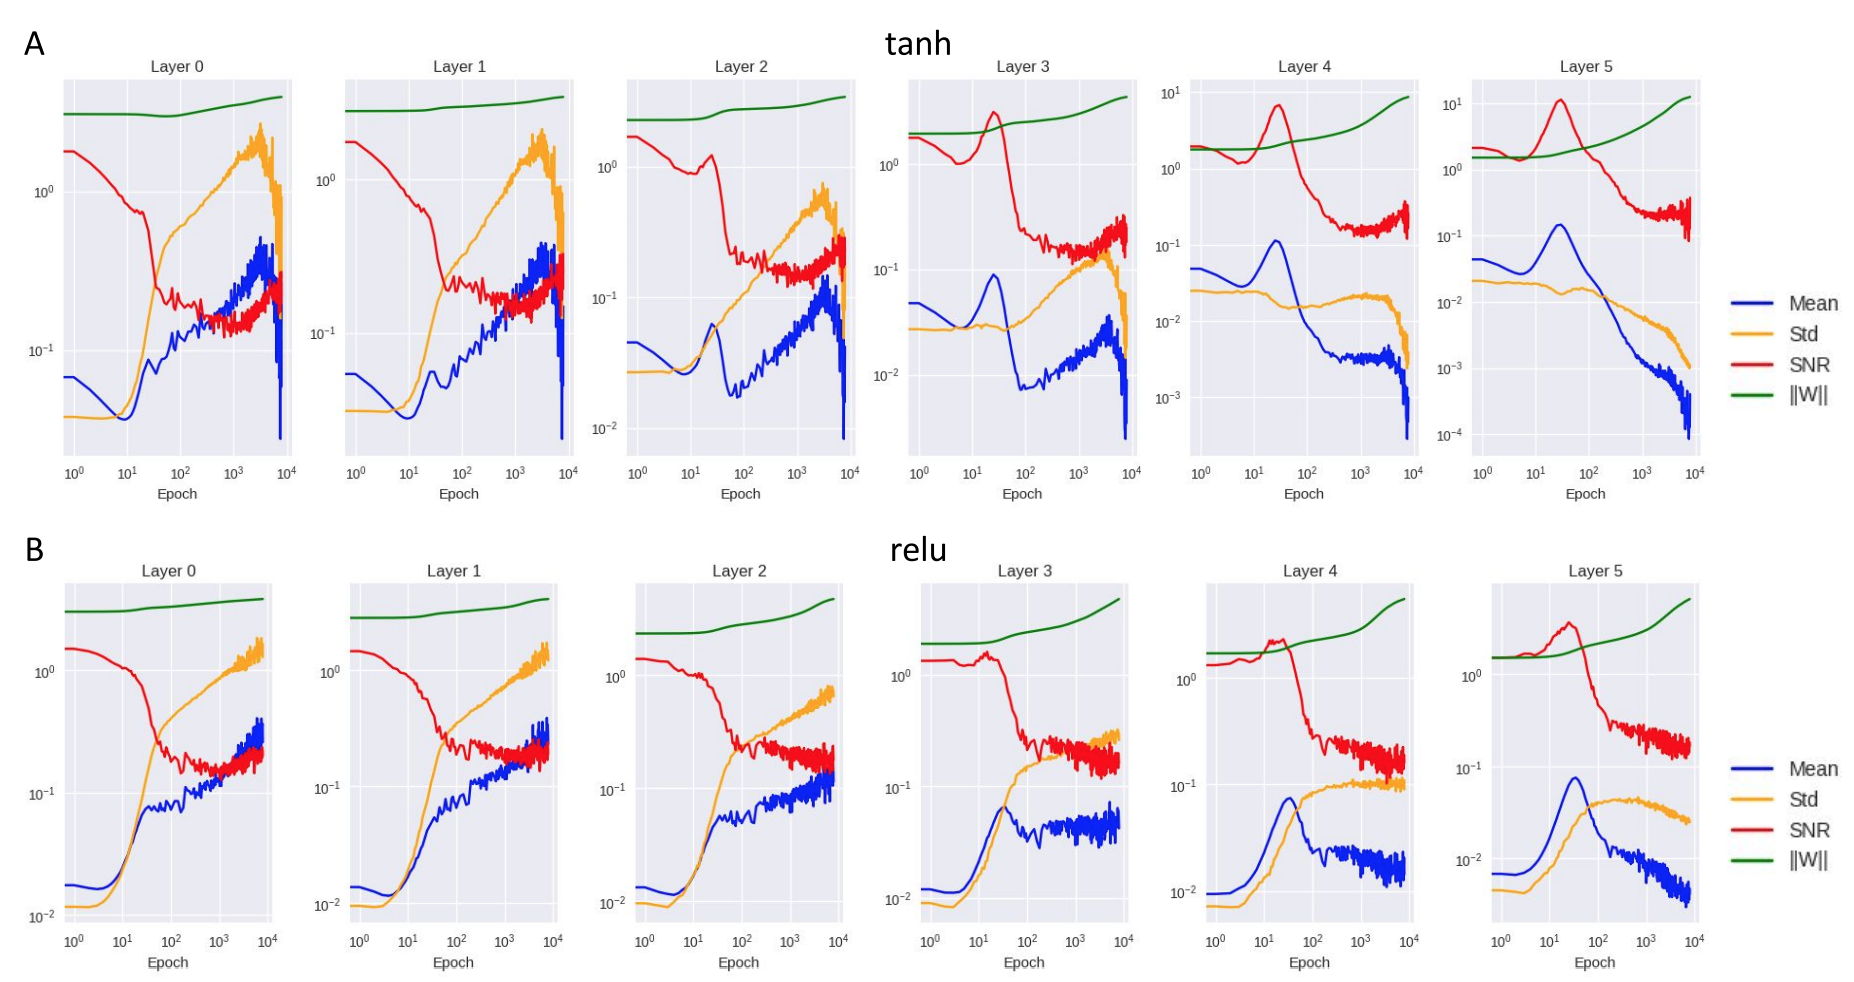
\includegraphics[width=0.8\textwidth]{sgd-snr.png}
\caption{Figure 20 from \cite{DL_and_IB_critics}: Gradient SNR phase transition. (A) tanh networks trained in the standard setting of SZT show a phase transition in every layer. (B) ReLU networks also show a phase transition in every layer, despite exhibiting no compression.}
\end{figure}

\subsection{Critics}
But there are two problems with their experiments:
\begin{itemize}
    \item Values of $I(X;Z_i)$ and $I(Y;Z_i)$ are either constant or infinite. That's why it's meaningless to measure them.
    \item Only toy experiments are performed. Authors claimed (in 2017) that they have CIFAR-10 experiments running, but no paper about this was published since.
    \item It does not work for ReLU, i.e. \cite{DL_and_IB_critics}. N.Tishby answer, that bad binning procedure was used, that's why authors got such results. But more sophisticated methods (Kraskov k-means and KDE) of estimating MI didn't lead to something better. Besides, they built ReLU network which exhibit right SNR behaviour, but didn't compress. 
\end{itemize}

\subsection{Why MI is either constant or infinite}
\begin{proposition}
Consider a discrete distribution $x \sim p(x)$ (possible with countable support) and a NN
\[
f(x) = \sigma(...\sigma(W_2\sigma(W_1 x + b_1) + b_2)...)
\]
with some injective non-linearity $\sigma$ (sigmoid, tanh, LeakyReLU, SELU, etc).
Then there is only measure-zero set of weights $W_1, ..., W_L, b_1, ..., b_L$ s.t. for some $x_i \neq x_j$ from $p(x)$ we get $f(x_i) = f(x_j)$.
This means, that NN is injective for $p(x)$.
\end{proposition}

\begin{proposition}
If NN is deterministic, then $I(z_l;x)$ is either constant (for descrete $x$) or infinite (for continuous $x$), regardless of training.
\end{proposition}

\begin{proof}
Consider a discrete setting. Then
\[
I(z_l;x) = H(x) - H(x|z_l)
\]

We are going to prove that $H(x|z_l) \equiv 0$:
\[
H(x|z_l) = H(x|x) = 0
\]
We used the fact that since $z_l$ is an injective and deterministic mapping of $x$, then we can invert it (it is clearly surjective by design: we use only support of $z_l$).

TODO: prove for continuous distribution.
Looks like we'll need local injectivity (which should work for ReLU too since they are piecewise-linear?).
And show that conditional entropy is $-\infty$ for some regions.
\end{proof}

\subsection{Remarks}
\begin{remark}
Authors in \cite{Estimating_MI_in_NNs} claim that we measure not MI, but some other quantity, connected to clusterization.
So although we have just proved that it's not possible for MI to change actually, another term is changing and it's changing for ReLU too.
Unfortunately, proofs about clusterization are only empirical (yet).
\end{remark}

\begin{remark}
Actually, their claims about SGD are hold true and are observed in other works.
\end{remark}

\begin{remark}
Actually, N.Tishby claims in his talk, that they have rigorous proofs about SGD behaviour and compression generalization bounds.
It was pusblished on ICLR 2019, but got somewhat ``retracted''.
\end{remark}


\section{Disentangled representations}

The following theorem gives us a hope to build invariant and disentangled representations.
Informally, it says that if we can build sufficient and minimal representations (which we are building by optimizing IB Lagrangian, for example), then we get invariant and disentangled ones.

\begin{proposition}
If $\eta$ is a nuisance for the task $y$ and $z$ is a sufficient representation of $x$ and we have a Markov chain $\eta \to x \to z$, then
\[
I(z;\eta) \leq I(z;x) - I(x;y)
\]

Moreover, if $y$ is discrete, then we can use task-decomposition lemma and prove something more strict:
\[
I(z;\eta) = I(z;x) - I(x;y) - \epsilon,
\]
where $\epsilon \triangleq I(z; y|\eta) - I(x;y)$.
\end{proposition}

\begin{proof}
As we have a Markov chain $(y,\eta) \to x \to z$ then by DPI $I(z;y,\eta) \leq I(z;x)$.
By chain rule we have
\[
I(z; \eta) = I(z; y, \eta) - I(z; y | \eta) \leq I(z;x) - I(z; y | \eta)
\]

By definition of nuisance $y \perp \eta$ so $I(z;y|\eta) \geq I(z;y)$, because (by one of identities for conditional MI):
\[
\begin{split}
I(z;y|\eta)
&= H(y|\eta) - H(y|z,\eta) \\
&= H(y) - H(y|z,\eta) \\
&\geq H(y) - H(y|z) \\
&= I(z;y)
\end{split}
\]

As $z$ is sufficient, i.e. $I(x;y) = I(z;y)$ we obtain
\[
I(z;\eta) \leq I(z;x) - I(z; y | \eta) \leq I(z;x) - I(z;y) = I(z;x) - I(x;y)
\]

Now consider, that we have $p(x;y)$ and $y$ is discrete.
Then by task-nuisance decomposition lemma we can introduce a nuisance $\eta$ s.t. $x = f(y;\eta)$ and $f$ is deterministic.
That's why we have
\[
I(z;x) = I(z; y, \eta) = I(z;\eta) + I(z; y | \eta)
\]
Rearranging terms we get
\[
I(z;\eta) = I(z;x) - I(x;y|\eta) = I(z;x) - I(x;y) - \underbrace{(I(x;y|\eta) - I(x;y))}_\varepsilon
\]

Let's prove that $0 \leq \varepsilon \leq H(y|x)$.
By definition of $\varepsilon$:
\begin{align*}
\varepsilon &= I(z;y|\eta) - I(x;y)
\shortintertext{Since $y|\eta \to x|\eta \to z|\eta$ is a Markov chain, then by DPI:}
&\leq I(x;y|\eta) - I(x;y) \\
&= H(y|\eta) - H(y|x,\eta) - H(y) + H(y|x) \\
&= H(y) - H(y|x,\eta) - H(y) + H(y|x) \\
&= H(y|x) - H(y|x,\eta) \\
%\shortintertext{Since $y$ is discrete and $H(y|x,\eta) \geq 0$:}
%\shortintertext{TODO: actually, to measure information-theoretic things between discrete and continuous r.v. we should convert discrete to delta-distribution, so $H(y|x,\eta)$ can be negative.}
\shortintertext{The last inequality is subtle, actually. We use the fact $H(y|x) - H(y|x,\eta) = I(y; \eta, x) \geq 0 \Rightarrow H(y|x) \geq H(y|x,\eta)$. And $\epsilon \geq 0$ follows from equation proved above: $I(z;y|\eta) \geq I(z;y) = I(x;y)$. That's why $H(y|x) \geq 0$, because it's a valid upper bound.}
&\leq H(y|x)
\end{align*}

\end{proof}

What does it give us? Does it give us invariance and disentanglement?
First of all, we see, that as more minimal our $z$ the more invariant it is, because minimal sufficient statistic implies that $I(x;z)$ is the most minimal possible!
And the first term is the only term we can influence with our $z$.

Unfortunately, it does not give us disentanglement yet.
To ensure disentanglement we need additional assumptions.
But before diving into it, let's think about how can we achieve invariance with what we already now?

\begin{corollary}
Minimizing IB Lagrangian with $\beta \to 0$
\[
H(y|z) + \beta I(x;z)
\]
\end{corollary}

\begin{proof}
This is true by theorem proved above.
\end{proof}

Introducing bottlenecks by adding noise or reducing dimensionality.
TODO: shouldn't we prove that bottlenecks reduces MI?
\begin{corollary}
Imagine we have a Markov chain $(y,\eta) \to x \to z_1 \to z_2$ and $I(z_1;z_2) < I(x; z_1)$, i.e. there is some bottleneck on the road between $z_1 \to z_2$. Then if $z_2$ is sufficient, it is more invariant    
\end{corollary}

\begin{proof}[Bottlenecks promote invaraince]
\begin{align*}
I(z_2;\eta) &\leq I(z_2;z_1) - I(z_1,y) = I(z_2; z_1) - I(x, y) < I(z_1; x) - I(x,y)
\end{align*}
\end{proof}

\begin{corollary}
Imagine setup above.
If $y$ is discrete and is a deterministic function of $x$, then inequality is strict.
\end{corollary}

\begin{proof}
We have
\[
\begin{split}
I(z_2; \eta) \leq I(z_2; z_1) - I(x;y) < I(z_1; x) - I(x;y) = I(z_1; \eta) + \varepsilon
\end{split}
\]
Since $y$ is a deterministic function of $x$ then $\varepsilon = 0$, hence the desired result.
\end{proof}

\begin{corollary}[Stacking increases invariance]
Consider we a have a Markov chain of layers
\[
(y,\eta) \to x \to z_1 \to ... \to z_l
\]
If $z_L$ is still sufficient, then it's more invariant.
\end{corollary}

TODO:
Well, this is because we have a Markov chain $\eta \to ... \to z_l$, it's not a corollary:
$I(\eta; z_l) \leq I(\eta; z_i)$.

\section{Information in the weights}
\subsection*{Information decomposition}
Consider a data distribution $(X,Y) = D \sim p(D|\theta)$.
We say that our model is:

\begin{equation}\label{eq:model-def}
p(D, \theta, w) = p(\theta) p(D|\theta) p_\phi(w| D)
\end{equation}

for some true unknown parameters $\phi$.
Here $p_\phi(w|D)$ is our distribution on the weights of NN --- it is not deterministic due to the randomness of the optimization process.
From this we can see that $p_\phi(w|D)$ is different from $p(w|D)$, which we would be computed if we'd have $p(D|w)$ to define our model (which is not).
This is a very big source of confusion.

If we have some weights and an input $X$, then our model defines a distribution $q(Y|X,w)$.
We want it to be as close as possible to $p(Y|X,w)$, which is computed from \eqref{eq:model-def}.

\begin{theorem}
Let $D = (X,Y)$ be a fixed dataset.
Then
\begin{equation}
H_{p,q}(Y|X,w) = \underbrace{H(Y|X,\theta)}_{\text{intrinsic error}} + \underbrace{I(\theta; Y | X,w)}_{\text{sufficiency}} + \underbrace{\expect[X,w]{\kl{p(Y|X,w)}{q(Y|X,w)}}}_{\text{efficiency}} - \underbrace{I(Y,w|X,\theta)}_{\text{overfitting}}
\end{equation}
\end{theorem}

\begin{proof}
Cross-entropy can be written as
\begin{equation}
\begin{split}
H_{p,q}(Y|X,w)
&= \expect[p(Y,X,w)]{-\log q(Y|X,w)}
\\
&= \expect[p(Y,X,w)]{-\log p(Y|X,w)} + \expect[p(Y,X,w)]{\log\frac{p(Y|X,w)}{q(Y|X,w}}
\\
&= H_p(Y|X,w) + \expect[X,w]{\kl{p(Y|X,w)}{q(Y|X,w)}}
\end{split}
\end{equation}

Let's prove the rest.
Since $I(X;Y|Z) = H(X|Z) - H(X|Y,Z)$ (analog of $I(X;Y) = H(X) - H(X|Y)$), we can see that:
\[
H_p(Y|X,w) = I(Y;\theta | X,w) + H(Y|X,w,\theta)
\]

Applying the same identity to $I(Y;w|X,\theta)$ we obtain
\[
H(Y|X,w,\theta) = H_p(Y|X,\theta) - I(Y;w|X,\theta)
\]
hence the desired result:
\[
H_p(Y|X,w) = I(Y;\theta | X,w) + H_p(Y|X,\theta) - I(Y;w|X,\theta)
\]
\end{proof}

Why do we call the terms so?
\begin{enumerate}
    \item $H(Y|X,\theta)$ --- intrinsic error: just some constant, which does not depend on $w$. This is the error we would get if we would know true data distribution.
    \item $I(\theta; Y | X,w)$ --- sufficiency: how much information does $w$ know about $\theta$ when it sees a dataset. Why is it so? Remember the definition of sufficiency that we had: $P(A|B,\psi) = P(A|B)$ which is equivalent to $I(A : \psi |B ) = H(A | B) - H(A | B, \psi) = 0$. Let's apply this to $p(Y|\theta, w, X)$. We want to measure $I(Y:\theta | w, X) = H(Y | w, X) - H(Y | \theta, w, X)$. If it is low, then we have $p(Y | \theta, w, X) \approx p(Y | w, X)$, i.e. $\theta$ is very well captured by $w$, i.e. $w$ is a sufficient statistic for $\theta$ of $Y$ (we assume, that we always know $X$). Besides, there is an often assumption about $p(X,\theta) = p(X)p(\theta)$, i.e. features $X$ are generated independently.
    \item $\expect[X,w]{\kl{p(Y|X,w)}{q(Y|X,w)}}$ --- efficiency: how efficient is it to use neural networks of the kind $f_w$ to approximate true data distribution. It shows how close our approximation $q(Y|X,w)$ is to a true $p(Y|X,w)$ data distribution, obtained from model \eqref{eq:model-def}.
    \item $I(Y,w|X,\theta)$ --- overfitting: shows, how much uninformative information does $w$ memorizes about $y$. Why it shows only uninformative information? Because in this term we assume that both $\theta$ and $X$ are known. So, imagine, that we know $\theta$ and $X$ --- this means, that we know everything good we can about $p(Y|X,\theta)$. But the weights $w$ are trying to memorize something more.
\end{enumerate}

So we see that NN can potentially solve the task (obtain good values of loss) just by maximizing overfitting term, i.e. memorizing the dataset.
So what we do is just adding a regularization term
\[
L(\phi) = H_{p,q}(Y|X,w) + \beta I(w;D)
\]
Note that this term is not the same thing as $I(w;y|\theta, X)$, but we cannot do better.

Unfortunately, $I(w;D)$ is intractable to compute (we need an expectation over all datasets and all training procedures), so we add an upper bound
\begin{equation}
\begin{split}
I(w; D) &= \expect[D]{\kl{p_\phi(w|D)}{p_\phi(w)}}
\\
&\leq \expect[D]{\kl{p_\phi(w|D)}{p_\phi(w)}} + \kl{p_\phi(w)}{p(w)}
\\
&= \expect[D]{\kl{p_\phi(w|D)}{p(w)}}
\end{split}
\end{equation}

Here $p(w)$ is any distribution on the weights.
We would like to take factorized distribution, so it's easier to compute: $p(w) = \prod p(w_i)$.
Ideally we would like to take factorized marginal $\prod p_\phi(w_i)$, because it's closest factorized distribution (TODO: prove it).
We could approximate this distribution by training model several times, but it's also costly and we just choose a (somewhat arbitrary) prior.
So, for some factorized prior $p(w) = \prod p(w_i)$ we have a loss
\[
L(\phi) = H_{p,q}(Y|X,w) + \beta \kl{p_\phi(w|D)}{p(w)}
\]

\subsection*{Model assumptions and upper bounding the loss}
We choose our $q(w|D)$ to be parametrized as
\[
w|D \sim \epsilon \hat{w}, \qquad \epsilon \sim \log \mathcal{N}()
\]

The main benefit of it is that $I(w;D)$ now can be written in closed form up to an arbitrary constant:
\[
123
\]

Authors say, that although this setup leads to arbitrary constant $C$, we could use truncated log-uniform or just gaussian multiplicative noise instead (in the former case MI would be intractable, but can be very closely approximated).

Our prior distribution $q(w)$ is factorized log-uniform:
\[
q(w) = \tilde{q}(w) = \prod_{i=1}^n q(w_i) \qquad q(w_i) = \frac{c}{|w_i|}
\]

\subsection*{Flat minima}
\begin{theorem}
Flat minima has low information.
\end{theorem}


\section{Mutual information estimators}
TBD.
%\subsection{Binning}
%
%\subsection{MINE}
%
%\subsection{MI estimator under gaussian convolutions}
%
%\subsection{EDGE}

\section{Appendix}
\subsection*{Why improper prior}
Uninformative prior is a prior which, rouhghly speaking, does not give any preferences in the r.v. values.
For finite discrete case uninformative prior is easy to define: it's just $P_i = 1/k$ where $k$ is the number of outcomes.
But what to do when our support is countable or continuous?

We can use improper priors as uninformative priors for continuous distributions.
For example, log-uniform prior.
Consider $p(\log x) = c$, or, which is equivalent:
\[
p(x) = p(\log x) \cdot \frac{d\log x}{dx} = c / x
\]

Authors say, that we can use improper prior for the weights and tell, that it is often the case in practice, referring the reader to their previous paper \cite{Information_Dropout}.
But in this paper they only showed that it's fine to use it for activations, not weights!

\subsection*{Kurtosis}
What is kurtosis (excess coefficient)?
\[
\gamma_2 = \text{Kurt}[X] = \frac{\expect{(X - \mu)^4}}{\sigma^4} - 3
\]
It shows, how ``picked'' our distribution is compared to $\mathcal{N}(0,1)$, which has zero kurtosis.
A similar notion is \textit{skeweness} (assymmetry coefficient), which is defined as
\[
\gamma_1 = \frac{\expect{(X - \mu)^3}}{\sigma^3}
\]
Symmetric distributions (with finite third moment) have skeweness of 0.


\section{Bibliography}
\printbibliography

\section*{Exercises}
\begin{enumerate}
%    \item Prove that
%\[
%\arg \min_{q(y)} \kl{p(x,y)}{p(x)q(y)} = f(y) \Longleftrightarrow f(y) = p(y)
%\]
    \item Prove that
\[
\arg \min_{q_1(x_1) , ... , q_n(x_n)} \kl{p(x_1, ..., x_n)}{q_1(x_1) \cdot ... \cdot q_n(x_n)} = p(x_1) \cdot ... \cdot p(x_n) \Longleftrightarrow q_1(x_1) , ... , q_n(x_n) = p(x_1), ..., p(x_n)
\]
%    \item We have a natural (which comes from our modeling) Markov property of $X \to Z \to Y$. Prove Markov property of $Z \to X \to Y$.
    \item Prove that if $X, Y$ are normally distributed, then $Z$ is normally distributed too. %http://www.jmlr.org/papers/volume6/chechik05a/chechik05a.pdf
    \item Maybe something on finding differential entropy of r.v. with infinite differential entropy. Or constructing such a variable.
    \item Prove that $I(X;T)$ is either infinity or constant (except measure zero of weights).
    \item Prove DPI
    \item IB solution is a minimal sufficient statistic (based on http://www.cs.huji.ac.il/labs/learning/Papers/ibgen.pdf, theorem 5)
\end{enumerate}

\end{document}
